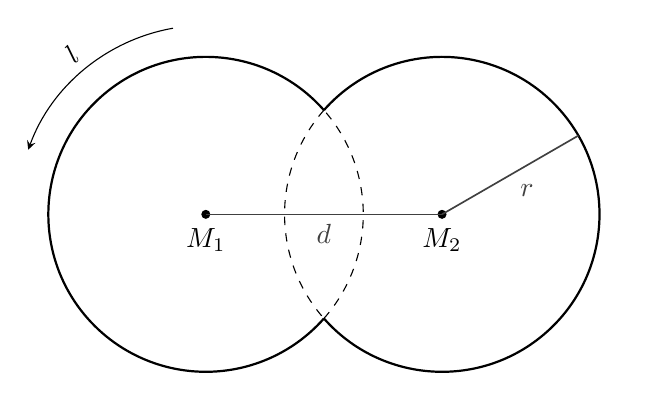
\begin{tikzpicture}[
    scale=2,
    >=stealth,
    point/.style = {draw, circle,  fill = black, inner sep = 1pt},
    dot/.style   = {draw, circle,  fill = black, inner sep = .2pt},
  ]
	\coordinate (R1) at (1,1); % Mittelpunkt des ersten Kreises
	\coordinate (R2) at (2.5,1); % Mittelpunkt des zweiten Kreises
	
	% Kreismittelpunkte
	\node (M1) at (R1) [point, label = {below:$M_1$}]{};
	\node (M2) at (R2) [point, label = {below:$M_2$}]{};
	
	% Bögen
	\draw[thick] (R1) ++(41.41:1) arc (41.41:318.59:1);
	\draw[dashed] (R1) ++(-41.41:1) arc (-41.41:41.41:1);
	\draw[thick] (R2) ++(221.41:1) arc (221.41:498.59:1);
	\draw[dashed] (R2) ++(138.59:1) arc (138.59:221.41:1);
	
	\draw[->] (R1) ++(100:1.2) arc (100:160:1.2) node[midway, sloped, above]{$l$};
	
	% Radius und Abstand der Kreise einzeichnen
	\draw[semithick,gray!50!black] (R2) -- node [below right] {$r$} +(30:1cm);
	\draw[semithick,gray!50!black] (R1) -- node [below] {$d$} (R2);
\end{tikzpicture}